\documentclass[../custom,grid]{flashcards}
%\usepackage{booktabs}
%\usepackage{array}
\usepackage{amsmath}
\usepackage{tikz}
\usepackage{float}
%\usepackage{enumitem}
%\usepackage{multirow}

\newcommand{\studyArea}{Risk Management Applications of Derivatives}

\def\labelitemii{$\circ$}
\def\labelitemiii{$\diamond$}
\def\labelitemiv{$\cdot$}

\begin{document}
\cardfrontstyle{headings}
\cardfrontfoot{Study Session 15}

\begin{flashcard}[\studyArea]{Number of Equity Futures Contracts Needed for a Target Portfolio Beta}
    \begin{flushleft}
        The formula for beta of a particular asset is $a$ is
        \begin{align*}
            \beta_a &= \frac{\text{cov}(a, M)}{\sigma^2_M}\\
            \\
            \text{where:}\\
            \text{cov}(a, M) &= \text{covariance of returns on asset $a$ with the market}\\
            \sigma^2_M &= \text{variance of the market returns}
        \end{align*}
        The number of contracts needed to achieve target portfolio beta, $\beta_T$, is
        \begin{align*}
            \text{number of contracts} &= \left ( \frac{\beta_T - \beta_P}{\beta_f} \right ) \left ( \frac{V_P}{P_f \times \text{multiplier}} \right )\\
            \\
            \text{where:}\\
            \beta_T &= \text{desired portfolio beta}\\
            \beta_P &= \text{portfolio beta}\\
            \beta_f &= \text{equity futures contract beta}\\
            V_P &= \text{current value of the portfolio}\\
            P_f &= \text{futures price}
        \end{align*}
    \end{flushleft}
\end{flashcard}

\begin{flashcard}[\studyArea]{Basic Form for Synthetic Equity or Synthetic Cash}
    \begin{flushleft}
        Synthetic cash or synthetic equity is modeled using long or short offsetting positions in equity futures.
        \begin{itemize}
            \item A synthetic risk-free asset is formed with a long stock position and a short stock index futures position.
            \item A synthetic equity position is formed with a long risk-free asset and a long stock index futures position.
        \end{itemize}
    \end{flushleft}
\end{flashcard}

\begin{flashcard}[\studyArea]{Number of Equity Futures Contracts Needed for Synthetic Cash Position}
    \begin{flushleft}
        An equity position can be converted to a synthetic cash position for $T$ years by using
        \begin{align*}
            \text{number of equity contracts} &= - \frac{V_P (1 + R_F)^T}{P_f}\\
            \\
            \text{where:}\\
            V_P &= \text{value of the equity position}\\
            P_f &= \text{total futures price (quoted price times multiplier)}\\
            R_F &= \text{risk-free rate}\\
            T &= \text{designated period of time}
        \end{align*}
    \end{flushleft}
\end{flashcard}

\begin{flashcard}[\studyArea]{Number of Futures Contracts Needed to Achieve for a Target Portfolio Duration}
    \begin{flushleft}
        \begin{align*}
            \text{number of contracts} &= (\text{yield beta}) \left ( \frac{\text{MD}_T - \text{MD}_P}{\text{MD}_F} \right ) \left ( \frac{V_P}{P_f \times \text{multiplier}} \right )\\
            \\
            \text{where:}\\
            V_P &= \text{current value of the portfolio}\\
            P_f &= \text{futures price}\\
            \text{MD}_T &= \text{target modified duration}\\
            \text{MD}_P &= \text{modified duration of the portfolio}\\
            \text{MD}_F &= \text{modified duration of the futures contract}
        \end{align*}
    \end{flushleft}
\end{flashcard}

\begin{flashcard}[\studyArea]{Steps to Synthetically Change Equity and Bond Allocations}
    \begin{itemize}
        \item To reallocate from equity to bonds
            \begin{enumerate}
                \item Remove all systematic risk (target a beta of zero) by shorting equity futures.
                \item Add duration to the position (target a modified duration of more than zero) by going long bond futures.
            \end{enumerate}
        \item To reallocate from bonds to equity
            \begin{enumerate}
                \item Remove all duration (target a modified duration of zero) by shorting bond futures.
                \item Add systematic risk to the position (target a beta of more than zero) by going long equity futures.
            \end{enumerate}
    \end{itemize}
\end{flashcard}

\begin{flashcard}[\studyArea]{Preinvesting}
    \begin{flushleft}
        Preinvesting is taking a long futures position to create an exposure converting a future cash inflow into a synthetic equity or bond position.
    \end{flushleft}
\end{flashcard}

\begin{flashcard}[\studyArea]{Three Types of Foreign Exchange Risk}
    \begin{enumerate}
        \item \textbf{Transaction exposure} is present when a cash flow in a foreign currency occurs at a future date. Can be hedged by selling forward in the case of a receipt or buying forward in the case of a payment.
        \item \textbf{Economic exposure} refers to situations when changes in currency value affect competitiveness. Some examples are companies that
            \begin{itemize}
                \item Export and sell products in foreign markets. Domestic currency appreciation means less competitive products internationally.
                \item Purchase and import from foreign markets. Domestic currency depreciation means costs in the domestic currency increase.
                \item Operate domestically, but have competitors or suppliers who are affected by changes in currency value.
            \end{itemize}
            This can be desirable to hedge, but difficult to quantify.
        \item \textbf{Translation exposure} is the risk of converting foreign financial statements into domestic currency units. Generally not hedged as it's not seen as a real cash flow risk.
    \end{enumerate}
\end{flashcard}

\begin{flashcard}[\studyArea]{Hedging Foreign Market and Foreign Currency Risks}
    \begin{itemize}
        \item Hedging foreign market risk
            \begin{itemize}
                \item Can sell short (sell forward) the foreign market index.
                \item The effectiveness depends on correlation of the portfolio and the market index. Perfect correlation will return the foreign risk-free rate.
                \item Applying a currency hedge on top of this will return the domestic risk-free rate.
            \end{itemize}
        \item Hedging foreign currency risk
            \begin{itemize}
                \item Problem is uncertainty of future value. Strategies to deal with this are
                \begin{itemize}
                    \item Hedge a minimum future value.
                    \item Hedge the estimated future value.
                    \item Hedge the initial value of the portfolio.
                \end{itemize}
            \end{itemize}
    \end{itemize}
\end{flashcard}

\begin{flashcard}[\studyArea]{Hedging with Forwards Versus Futures}
    \begin{itemize}
        \item Practical differences
            \begin{itemize}
                \item Futures are standardized while forwards are customized.
                \item Forwards have counterparty risk while futures use clearinghouses.
                \item Futures are more regulated and transparent.
                \item Futures require margin.
            \end{itemize}
        \item Empirical differences
            \begin{itemize}
                \item Most bond and equity hedging is done with futures, but this creates cross-hedge and basis risk.
                \item Interest payment and currency hedges usually use forwards so exact amounts and dates can be hedged.
                \item Eurodollar futures are a large market that is mostly used by dealers and market makers to hedge their own business needs.
            \end{itemize}
    \end{itemize}
\end{flashcard}

\begin{flashcard}[\studyArea]{Covered Call}
    \begin{flushleft}
        Buy the underlying and sell a call option. Used to generate income when the underlying price is expected to remain unchanged.
        \begin{center}
            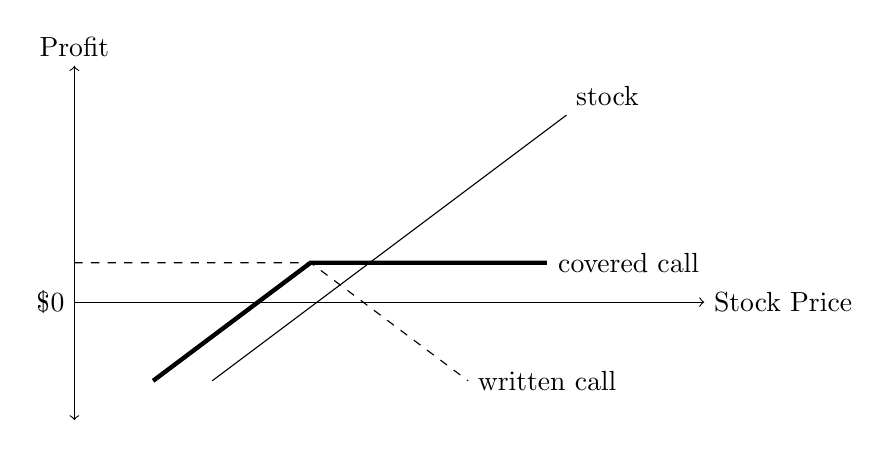
\begin{tikzpicture}
                \draw[<->] (0, -1.5) -- (0, 3) node[above] {Profit};
                \draw[->] (0, 0) node[left] {\$0} -- (8, 0) node[right] {Stock Price};
                \draw[dashed] (0, 0.5) -- (3, 0.5) -- (5, -1) node[right] {written call};
                \draw[ultra thick] (1, -1) -- (3, 0.5) -- (6, 0.5) node[right] {covered call};
                \draw (1.75, -1) -- (6.25, 2.375) node[above right] {stock};
            \end{tikzpicture}
        \end{center}
        \begin{align*}
            \text{profit} &= -\max(0, S_T - X) + S_T - S_0 + C_0\\
            \text{maximum profit} &= X + C_0 - S_0\\
            \text{maximum loss} &= S_0 - C_0\\
            \text{breakeven price} &= S_0 - C_0
        \end{align*}
    \end{flushleft}
\end{flashcard}

\begin{flashcard}[\studyArea]{Protective Put}
    \begin{flushleft}
        Buy the underlying and buy a put option. Limits downside risk at the cost of the put premium, $P_0$.
        \begin{center}
            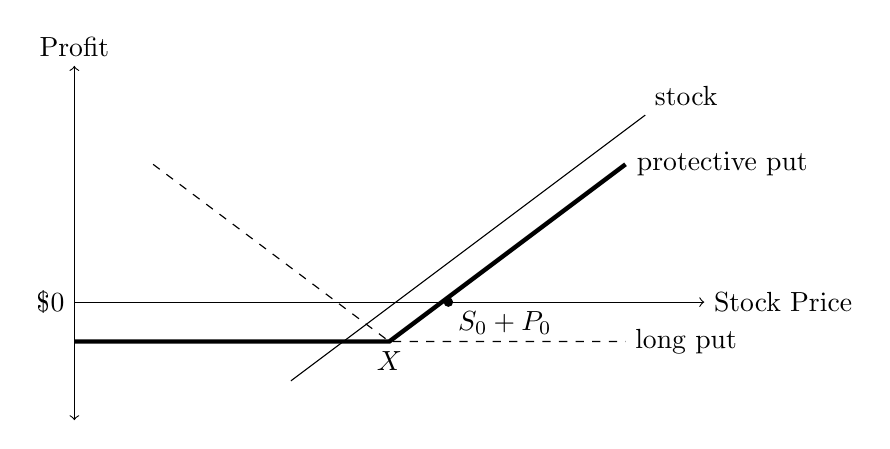
\begin{tikzpicture}
                \draw[<->] (0, -1.5) -- (0, 3) node[above] {Profit};
                \draw[->] (0, 0) node[left] {\$0} -- (8, 0) node[right] {Stock Price};
                \draw[dashed] (1, 1.75) -- (4, -0.5) -- (7, -0.5) node[right] {long put};
                \draw[ultra thick] (0, -0.5) -- (4, -0.5) -- (7, 1.75) node[right] {protective put};
                \draw (2.75, -1) -- (7.25, 2.375) node[above right] {stock};
                \node[below] at (4, -0.5) {$X$};
                \draw[fill] (4.75, 0) circle[radius=1.5pt] node[below right] {$S_0 + P_0$};
            \end{tikzpicture}
        \end{center}
        \begin{align*}
            \text{profit} &= \max(0, X - S_T) + S_T - S_0 - P_0\\
            \text{maximum profit} &= S_T - S_0 - P_0\\
            \text{maximum loss} &= S_0 - X + P_0\\
            \text{breakeven price} &= S_0 + P_0
        \end{align*}
    \end{flushleft}
\end{flashcard}

\begin{flashcard}[\studyArea]{Bull Spread}
    \begin{flushleft}
        Purchase a call option with a low exercise price, $X_L$ and sell a call with a higher exercise price, $X_H$. At inception, $X_L < X_H$ and $C_{L, 0} < C_{H, 0}$. The investor expects the stock price to end up between $X_L$ and $X_H$. This provides limited upside if the stock rises, with a limited downside.
        \begin{center}
            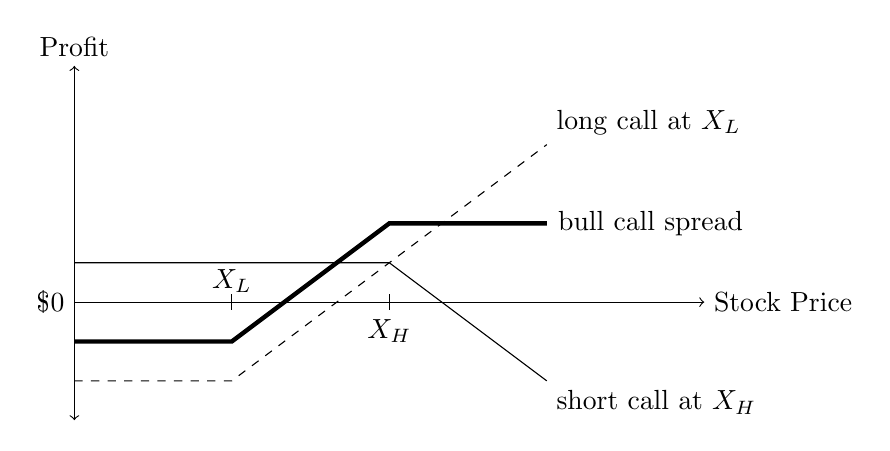
\begin{tikzpicture}
                \draw[<->] (0, -1.5) -- (0, 3) node[above] {Profit};
                \draw[->] (0, 0) node[left] {\$0} -- (8, 0) node[right] {Stock Price};
                \draw[dashed] (0, -1) -- (2, -1) -- (6, 2) node[above right] {long call at $X_L$};
                \draw[ultra thick] (0, -0.5) -- (2, -0.5) -- (4, 1) -- (6, 1) node[right] {bull call spread};
                \draw (0, 0.5) -- (4, 0.5) -- (6, -1) node[below right] {short call at $X_H$};
                \draw (2, 0.1) -- (2, 0) node [above] {$X_L$} -- (2, -0.1);
                \draw (4, 0.1) -- (4, -0.1) node[below] {$X_H$};
            \end{tikzpicture}
        \end{center}
        \begin{align*}
            \text{profit} &= \max(0, S_T - X_L) - \max(0, S_T - X_H) - C_{L, 0} + C_{H, 0}\\
            \text{maximum profit} &= X_H - X_L - C_{L, 0} + C_{H, 0}\\
            \text{maximum loss} &= C_{L, 0} - C_{H, 0}\\
            \text{breakeven price} &= X_L + C_{L, 0} - C_{H, 0}
        \end{align*}
    \end{flushleft}
\end{flashcard}

\begin{flashcard}[\studyArea]{Bear Spread}
    \begin{flushleft}
        Sell a call with a low exercise price, $X_L$ and buy a call with a higher exercise price, $X_H$. This provides limited upside if the stock falls, with a limited downside. As prices fall, the investor keeps the premium of the written call, net of the long call premium.
        \begin{center}
            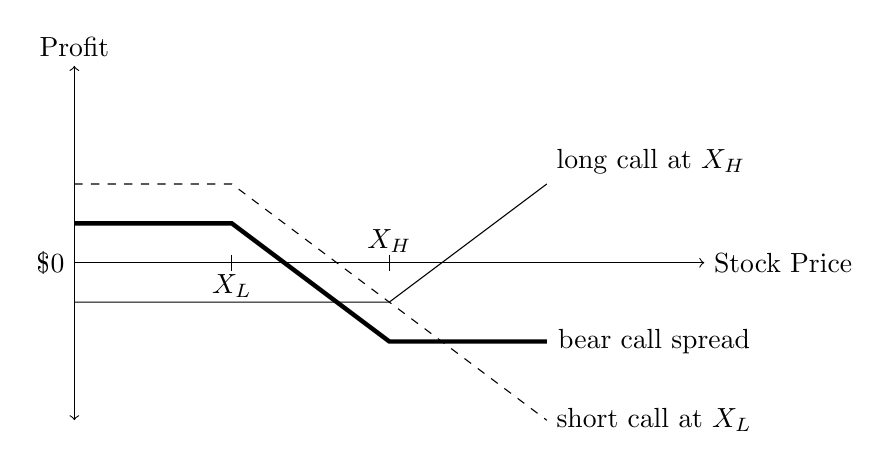
\begin{tikzpicture}
                \draw[<->] (0, -2) -- (0, 2.5) node[above] {Profit};
                \draw[->] (0, 0) node[left] {\$0} -- (8, 0) node[right] {Stock Price};
                \draw[dashed] (0, 1) -- (2, 1) -- (6, -2) node[right] {short call at $X_L$};
                \draw[ultra thick] (0, 0.5) -- (2, 0.5) -- (4, -1) -- (6, -1) node[right] {bear call spread};
                \draw (0, -0.5) -- (4, -0.5) -- (6, 1) node[above right] {long call at $X_H$};
                \draw (2, 0.1) -- (2, -.03) node [below] {$X_L$} -- (2, -0.1);
                \draw (4, 0.1) -- (4, 0) node[above] {$X_H$} -- (4, -0.1);
            \end{tikzpicture}
        \end{center}
        \begin{align*}
            \text{profit} &= \max(0, S_T - X_H) - \max(0, S_T - X_L) + C_{L, 0} - C_{H, 0}\\
            \text{maximum profit} &= X_H - X_L + C_{L, 0} - C_{H, 0}\\
            \text{maximum loss} &= C_{L, 0} - C_{H, 0}\\
            \text{breakeven price} &= X_L + C_{L, 0} - C_{H, 0}
        \end{align*}
    \end{flushleft}
\end{flashcard}

\begin{flashcard}[\studyArea]{Butterfly Spread with Calls}
    \begin{flushleft}
        Buy two calls at strike prices $X_L$ and $X_H$ and write two calls at strike price $X_M$ with $X_L < X_M < X_H$. The investor expects the stock price to stay near $X_M$, but the downside loss is limited by the purchased calls.
        \begin{center}
            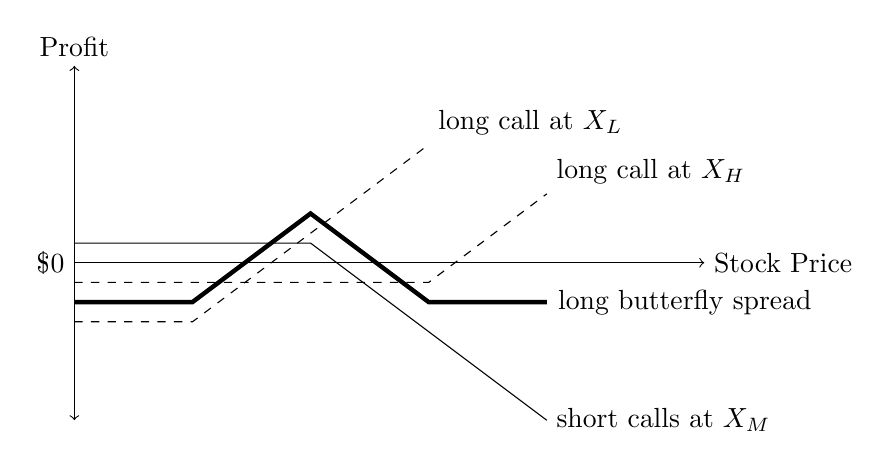
\begin{tikzpicture}
                \draw[<->] (0, -2) -- (0, 2.5) node[above] {Profit};
                \draw[->] (0, 0) node[left] {\$0} -- (8, 0) node[right] {Stock Price};
                \draw[dashed] (0, -0.25) -- (4.5, -0.25) -- (6, 0.875) node[above right] {long call at $X_H$};
                \draw[dashed] (0, -0.75) -- (1.5, -0.75) -- (4.5, 1.5) node[above right] {long call at $X_L$};
                \draw[ultra thick] (0, -0.5) -- (1.5, -0.5) -- (3, 0.625) -- (4.5, -0.5) -- (6, -0.5) node[right] {long butterfly spread};
                \draw (0, 0.25) -- (3, 0.25) -- (6, -2) node[right] {short calls at $X_M$};
            \end{tikzpicture}
        \end{center}
        \begin{align*}
            \text{profit} &= \max(0, S_T - X_L) - 2 \max(0, S_T - X_M)\\
            &+ \max(0, S_T - X_H) - C_{L, 0} + 2C_{M, 0} - C_{H, 0}\\
            \text{maximum profit} &= X_M - X_L - C_{L, 0} + 2C_{M, 0} - C_{H, 0}\\
            \text{maximum loss} &= C_{L, 0} - 2 C_{M, 0} + C_{H, 0}\\
            \text{breakeven price} &= X_L + C_{L, 0} - 2C_{M, 0} + C_{H, 0} \text{ and } 2X_M - X_L - C_{L, 0} + 2C_{M, 0} - C_{H, 0}\\
        \end{align*}
    \end{flushleft}
\end{flashcard}

\begin{flashcard}[\studyArea]{Straddle}
    \begin{flushleft}
        Buy both a put and a call with the same strike price and expiration on the same asset. The investor expects a large price move in some direction, and will incur a loss if the price remains static.
        \begin{center}
            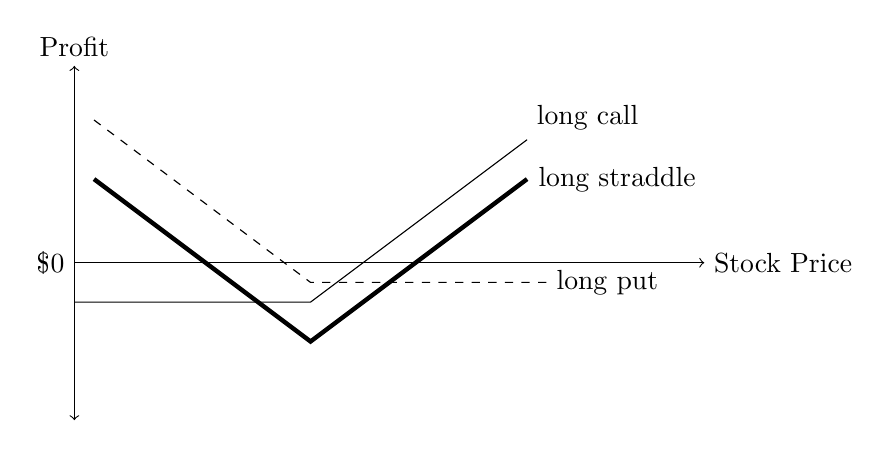
\begin{tikzpicture}
                \draw[<->] (0, -2) -- (0, 2.5) node[above] {Profit};
                \draw[->] (0, 0) node[left] {\$0} -- (8, 0) node[right] {Stock Price};
                \draw[dashed] (0.25, 1.8125) -- (3, -0.25) -- (6, -0.25) node[right] {long put};
                \draw (0, -0.5) -- (3, -0.5) -- (5.75, 1.5625) node[above right] {long call};
                \draw[ultra thick] (0.25, 1.0625) -- (3, -1) -- (5.75, 1.0625) node[right] {long straddle};
            \end{tikzpicture}
        \end{center}
        \begin{align*}
            \text{profit} &= \max(0, S_T - X) + \max(0, X - S_T) - C_0 - P_0\\
            \text{maximum profit} &= S_T - X - C_0 - P_0\\
            \text{maximum loss} &= C_0 + P_0\\
            \text{breakeven price} &= X - C_0 - P_0 \text{ and } X + C_0 + P_0
        \end{align*}
    \end{flushleft}
\end{flashcard}

\begin{flashcard}[\studyArea]{Collar}
    \begin{flushleft}
        Combination of a protective put and a covered call. Can be zero-cost if call and put premia are equal. Usually put has lower strike $X_L$ and call has higher strike $X_H$. Both the upside and downside are limited by the call and the put respectively.
        \begin{center}
            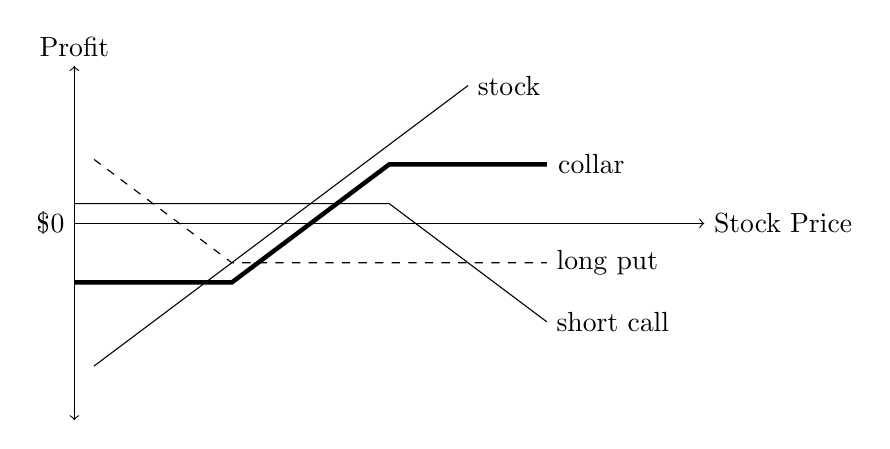
\begin{tikzpicture}
                \draw[<->] (0, -2.5) -- (0, 2) node[above] {Profit};
                \draw[->] (0, 0) node[left] {\$0} -- (8, 0) node[right] {Stock Price};
                \draw[dashed] (0.25, 0.8125) -- (2, -0.5) -- (6, -0.5) node[right] {long put};
                \draw (0, 0.25) -- (4, 0.25) -- (6, -1.25) node[right] {short call};
                \draw[ultra thick] (0, -0.75) -- (2, -0.75) -- (4, 0.75) -- (6, 0.75) node[right] {collar};
                \draw (0.25, -1.8125) -- (5, 1.75) node[right] {stock};
            \end{tikzpicture}
        \end{center}
        \begin{align*}
            \text{profit} &= \max(0, X_L - S_T) - \max(0, S_T - X_H) + S_T - S_0\\
            \text{maximum profit} &= X_H - S_0\\
            \text{maximum loss} &= S_0 - X_L\\
            \text{breakeven price} &= S_0
        \end{align*}
    \end{flushleft}
\end{flashcard}

\begin{flashcard}[\studyArea]{Box Spread}
    \begin{flushleft}
        Combination of a bull call spread and a bear put spread. That is, a long call and short put at $X_L$ and a long put and a short call at $X_H$. The payoff is always the same, regardless of the underlying price, which means assuming the prices are correct, the payoff is the risk-free rate.
        \begin{center}
            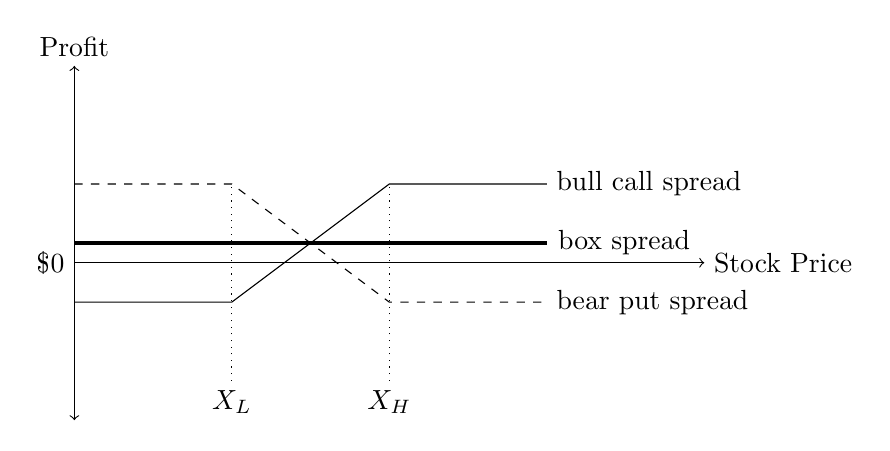
\begin{tikzpicture}
                \draw[<->] (0, -2) -- (0, 2.5) node[above] {Profit};
                \draw[->] (0, 0) node[left] {\$0} -- (8, 0) node[right] {Stock Price};
                \draw[dashed] (0, 1) -- (2, 1) -- (4, -0.5) -- (6, -0.5) node[above, right] {bear put spread};
                \draw (0, -0.5) -- (2, -0.5) -- (4, 1) -- (6, 1) node[above, right] {bull call spread};
                \draw[ultra thick] (0, 0.25) -- (6, 0.25) node[below, right] {box spread};
                \draw[dotted] (2, -1.5) node[below] {$X_L$} -- (2, 1);
                \draw[dotted] (4, -1.5) node[below] {$X_H$} -- (4, 1);
            \end{tikzpicture}
        \end{center}
    \end{flushleft}
\end{flashcard}
\end{document}
